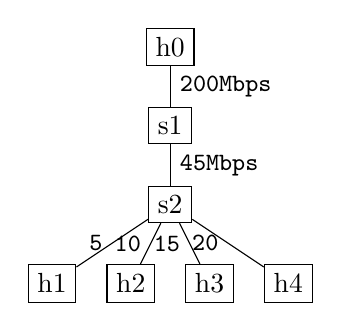
\begin{tikzpicture}
    \tikzstyle{host}=[draw]
    \tikzstyle{switch}=[draw]
    \tikzstyle{connection}=[]
    \tikzstyle{constr}=[right,font=\ttfamily\small]
    \node [host] (h0) at (0,4) {h0};
    \node [switch] (s1) at (0,3) {s1};
    \node [switch] (s2) at (0,2) {s2};
    \node [host] (h2) at (-0.5,1) {h2};
    \draw (h0) edge node [constr] {200Mbps} (s1);
    \draw (s1) edge node [constr] {45Mbps} (s2);
    \draw (s2) edge node [constr,left] {10} (h2);
	\node[host] (v1) at (-1.5,1) {h1};
	\node[host] (v2) at (0.5,1) {h3};
\draw  (s2) edge node [constr,left] {5} (v1);
\draw  (s2) edge node [constr,left] {15} (v2);
\node [host] (v3) at (1.5,1) {h4};
\draw  (s2) edge node [constr,left] {20} (v3);
\end{tikzpicture}